\documentclass[a4paper,12pt,nottoc]{article}
\usepackage{graphicx}
\usepackage[left = 3cm, right = 2cm, top = 2cm, bottom = 2cm]{geometry}
\usepackage{makecell}
\usepackage{booktabs}
\usepackage[justification=centering]{caption}
\usepackage{listings}
\usepackage{color}
\usepackage{xcolor}
\usepackage{hyperref}
\usepackage{tocbibind}
\usepackage{amsmath}
\usepackage{siunitx}
\usepackage{mhchem}
\hypersetup{
    colorlinks=true,
    linkcolor=blue,
    filecolor=blue,      
    urlcolor=blue,
    citecolor=blue,
}

\begin{document}

\begin{center}{\LARGE Detecting Fake News with Supervised Learning}\\\vspace{.5cm}Benjamin R. Perucco\\\vspace{.25cm}December 30, 2020\end{center}

\section{Definition}

\subsection{Project Overview}

Our world is highly interconnected and it is of paramount importance that citizens are informed objectively and truthfully about issues that influence and shape our world (like issues on geopolitics or climate change). The internet lead to a rise of news media (for example social media, news portals, etc.) to report on these stories. The vast amount of (online) news articles available yield a new phenomenon called fake news. Fake news is false or misleading information presented as news and can reduce the impact of real news \cite{bib:fakenews}. 

\subsection{Problem Statement}

This work is about answering the question whether machine learning (ML) can be applied to classify news articles as truthful or fake. There are several papers available where Ahmed et al. classified news articles \cite{bib:ahmed-2017} or hotel guest reviews \cite{bib:ahmed-2018} to be truthful or fake. Ahmed et al. used natural language processing (NLP) models to transform text into a structured, mathematical representation and achieved accuracies up to 92\% \cite{bib:ahmed-2017}.\\

\noindent Based on a set of features $\{f_{1}, f_{2}, f_{3}, ... \}$ extracted from news articles, a machine learning algorithm needs to be trained to find the relationship $\hat{\theta}$ between the a priori known classification of the news articles $y$ ($=0$ for truthful and $=1$ for fake) and the set of extracted features $\{f_{1}, f_{2}, f_{3}, ... \}$. The relation can be written as

\begin{gather}
\hat{y} =\hat{\theta}(X)
\end{gather}

\noindent where $\hat{y}$ is the predicted class label by the trained function $\hat{\theta}$ applied to a feature matrix $X$ that holds the set of features $\{f_{1}, f_{2}, f_{3}, ... \}$. $\hat{\theta}$ must be trained on available data, such that

\begin{gather}\label{eq:sse}
\sum_{i=1}^{n} \left(y - \hat{y} \right)^2
\end{gather}

\noindent is minimal. Here it is assumed that we have $n$ news articles where it is already known whether they are truthful or not.\\

\noindent A first step to be worked on is to extract a feature matrix $X$ from a set of news articles (or also called documents). How reliable is the prediction of class labels on unseen news articles once the function $\hat{\theta}$ has been found?

\subsection{Metrics}

Equation \ref{eq:sse} is rather used for regression problems where the predicted output is a continuous variable. For classification problems like news article classification into a truthful ($= 0$) or a fake class ($= 1$), the accuracy is a more suitable metric. This can be nicely demonstrated by the confusion matrix

\begin{gather}
\begin{bmatrix}
& 1 & 0 \\
1 & \textrm{TP} & \textrm{FP} \\
0 & \textrm{FN} & \textrm{TN}
\end{bmatrix}.
\end{gather}

\noindent The entries in the row indicate predicted class labels and the entries in the columns represent the real class labels. TP stands for true positives, TN for true negatives, FP for false positives and FN for false negatives. To asses the performance of $\hat{\theta}$, the accuracy $a$ is considered, which can be calculated as

\begin{gather}\label{eq:acc}
a = \frac{\textrm{TP} + \textrm{TN}}{\textrm{TP} + \textrm{TN} + \textrm{FN} + \textrm{FP}}.
\end{gather}

\section{Analysis}

\subsection{Algorithms and Techniques}

News articles must be converted into a structured, mathematical representation in order to be used by machine learning techniques. The following chapters discuss how we can convert text into numerical features.

\subsubsection{n-gram Model}

The $n$-gram is usually defined as a contiguous sequence of words with length $n$. For example, if $n = 1$, we speak of a unigram that contains only single words. Or if $n = 2$, we denote this as a bigram which is built on two adjacent words.\\

\noindent Consider the following text: ``Sometimes we eat green apples, and sometimes, the apples we eat are red.'' Based on a unigram (1-gram), we obtain a set of tokens: $\{$'sometimes', `we', `eat', `apples', `green', `and', `the', `are', `red'$\}$. We can derive a frequency array of tokens in the text: [2, 2, 2, 2, 1, 1, 1, 1, 1]. For the bigram (2-gram), another set of tokens is obtained: $\{$'sometimes we', `we eat', `eat green', `green apples', `apples and', `and sometimes', `sometimes the', `the apples', `apples we', `eat are', `are red'$\}$. The corresponding frequency array of tokens in the text is: [1, 1, 1, 1, 1, 1, 1, 1, 1, 1, 1]. Please note that punctuation is not considered when converting text into tokens.\\

\noindent In order to a build frequency arrays for a set of texts (or documents), a common vocabulary needs to be built of which the $n$-gram model is underlying principle.

\clearpage
\subsubsection{Vocabulary}

Consider a corpus $D$ which contains a set of documents $\{d_1, d_2, d_3, ..., d_n\}$. Then a vocabulary $F$ is a set of tokens $\{f_1, f_2, f_3, ..., f_m\}$ extracted from the corpus $D$. Mind that a token is created based on the $n$-gram model. Usually for a set of tokens, only the $m$ mostly occurring tokens in a corpus $D$ are considered. In the following, the tokens are denoted as features as these construct the features (or independent variables) of a machine learning model.\\

\subsubsection{Definitions}

Let $\sigma(d_i, f_j)$ denote the number of occurrences of feature $f_j$ in document $d_i$. Then a feature matrix $S$ can be built, where

\begin{gather}
S =
\begin{bmatrix}
\sigma(d_1, f_1) & \sigma(d_1, f_2) & \sigma(d_1, f_3) & ... & \sigma(d_1, f_m) \\
\sigma(d_2, f_1) & \sigma(d_2, f_2) & \sigma(d_2, f_3) & ... & \sigma(d_2, f_m) \\
\sigma(d_3, f_1) & \sigma(d_3, f_2) & \sigma(d_3, f_3) & ... & \sigma(d_3, f_m) \\
... & ... & ... & ... & ... & \\
 \sigma(d_n, f_1) & \sigma(d_n, f_2) & \sigma(d_n, f_3) & ... & \sigma(d_n, f_m)
\end{bmatrix}.
\end{gather}

\noindent An element $\sigma(d_i, f_j)$ in matrix $S$ (representing the document $d_i$ and feature $f_j$) is abbreviated using the notation $\sigma_{ij}$ for simplicity.

\subsubsection{Term Frequency Model}

The matrix $S$ could be already used for machine learning. Features usually need to be normalized in machine learning to increase performance. Therefore, the term frequency (TF) model normalizes matrix $S$ leading to matrix $\hat{S}$. An element $\hat{\sigma}_{ij}$ of matrix $\hat{S}$ is written as

\begin{gather}\label{eq:tf}
\hat{\sigma}_{ij} = \frac{\sigma_{ij}}{\sum_{j=1}^{m}\sigma_{ij}}.
\end{gather}

\noindent Or spoken in plain language: the number of occurrences of a feature $f_j$ in a document $d_i$ is divided by the total number of occurrences of all features $\{f_1, f_2, f_3, ..., f_m\}$ in the same document $d_i$. So we end up with a representation where the importance of each feature can be compared to other features in the same document (relative importance).

\subsubsection{Inverse Document Frequency Model}

The inverse document frequency (IDF) model is used to define the feature importance not just in a document $d_i$ but also compare its importance to the whole corpus $D$. A matrix $E$ is introduced, where an element $\epsilon_{ij}$ of matrix $E$ is $1$ if $\hat{\sigma}_{ij} > 0$ (or $\sigma_{ij} > 0$). An inverse normalization is applied to the matrix $E$ resulting in a vector $\hat{e}$. An element $\hat{\epsilon}_{j}$ of vector $\hat{e}$ is calculated as

\begin{gather}\label{eq:idf}
\hat{\epsilon}_{j} = 1 + \textrm{log}\left[\frac{|D|}{\sum_{i=1}^{n}\epsilon_{ij}}\right].
\end{gather}

\noindent Or spoken in plain language: in a corpus $D$ which comprises of a set of documents $\{d_1, d_2, d_3, ..., d_n\}$, it is counted in how many documents the feature $f_j$ appears. This number is used to divide the number of documents $|D|$ in a corpus $D$. Consider two examples: if a feature $f_j$ occurs in each document $\{d_1, d_2, d_3, ..., d_n\}$, we divide the number of documents $|D|$ in a corpus $D$ by the same number. So equation \ref{eq:idf} results in $1$, weighting feature $f_j$ as $1$. On the other hand, if a feature $f_j$ occurs only in one document, equation \ref{eq:idf} results in a much larger number, thus increasing the weight of feature $f_j$ in the corpus $D$.\\

\noindent Finally, a matrix $\hat{P}$ is obtained as the element-wise product of the term frequency matrix $\hat{S}$ and the inverse document frequency vector $\hat{e}$, written as $\hat{P} = \hat{S} \odot \hat{e}$. For an element $\hat{\pi}_{ij}$ of matrix $\hat{P}$, this is written as

\begin{gather}\label{eq:tf-idf}
\hat{\pi}_{ij} = \hat{\sigma}_{ij} \cdot \hat{\epsilon}_{j},\;\;\textrm{element-wise for}\;j = 1, 2, 3, ..., m .
\end{gather}

\noindent This term is denoted as the term frequency inverse document frequency (TF-IDF) model.

\subsection{Data Exploration}

A set of truthful and fake news articles is available on kaggle.com \cite{bib:kaggle}. The data was collected from real world sources. Truthful articles were obtained from Reuters and fake news articles were gathered from unreliable websites that were flagged by Politifact which is a fact-checking organization. These data sets contain different types of articles on different topics, the majority of articles focus on political and world news topics \cite{bib:ahmed-2018}.\\

\noindent There are 44,898 articles in total in the corpus. 21,417 of the articles are classified as truthful and 23,481 are classified as fake, so both class labels are roughly balanced. Approximately 6,169 of the articles are not unique. The duplicates are being removed after text processing discussed in chapter \ref{chap:data-preproc}.

\subsubsection{Visual Analysis of Top Features}

A first glimpse of the top 20 unigrams per class is given in figure \ref{fig:top20}. It can be observed from the unigrams that probably the most discussed topic in the set of news articles is the presidential election in the U.S. during the year 2016. Despite some unigrams that are used frequently in both classes of articles (like said, trump, presid, republican, etc.), we also see distinct unigrams only used in one class of articles. 

\clearpage
\section{Methodology}

\subsection{Data Preprocessing}\label{chap:data-preproc}

Raw text has to be brought into a clean state in order for feature extraction. Several text cleansing steps are performed like removal of introductory statements, dates, hyperlinks, numbers and stop words. Finally, so called stemming is performed to end up with the stem of a word (for example cat should identify such strings as cats, catlike, or catty \cite{bib:stemming}).

\begin{figure}[h]
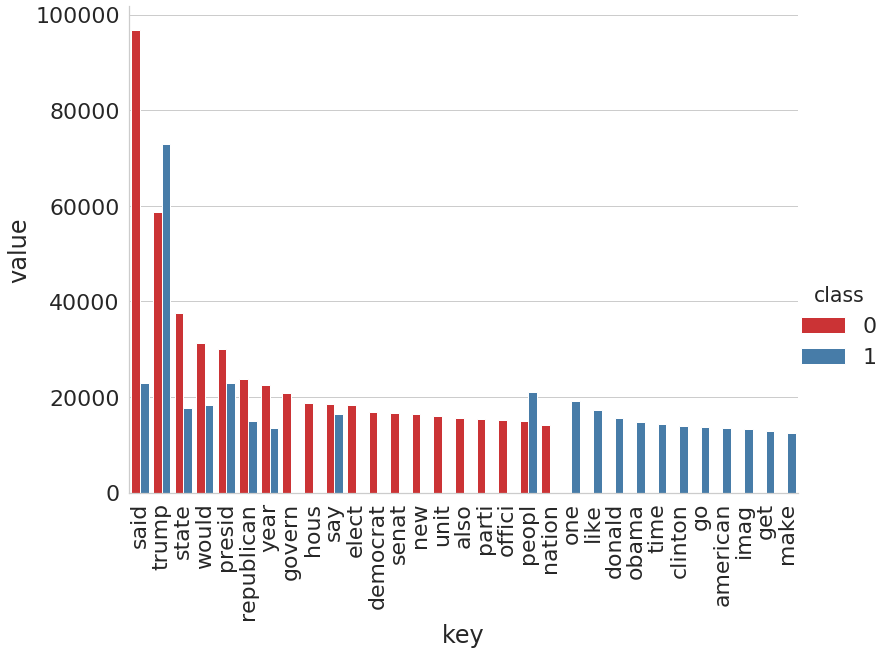
\includegraphics[width=14cm]{output/word_analysis_1.png}
\centering
\caption{Frequency of the top 20 unigrams per class extracted from the corpus.}\label{fig:top20}
\end{figure}

\subsection{Implementation}

\subsubsection{Feature Extraction Method}

The indices of the corpus are randomized and splitted into three different data sets as displayed in the table \ref{tab:datapreproc} below.

\begin{table}[h]
\begin{center}
\begin{tabular}{| l | l | r | c | c | c |}
\hline
Name & Purpose & Size & TF & IDF & TF-IDF \\
\hline
Training & Model training & 60\% & $\hat{S}_{\textrm{train}}$ & $\hat{E}_{\textrm{train}}$ & $\hat{S}_{\textrm{train}} \odot \hat{E}_{\textrm{train}}$ \\  
Test & Hyper parameter tuning & 20\% & $\hat{S}_{\textrm{test}}$ & $\hat{E}_{\textrm{train}}$ & $\hat{S}_{\textrm{test}} \odot \hat{E}_{\textrm{train}}$ \\    
Validation & Model validation & 20\% & $\hat{S}_{\textrm{valid}}$ & $\hat{E}_{\textrm{train}}$ & $\hat{S}_{\textrm{valid}} \odot \hat{E}_{\textrm{train}}$ \\
\hline 
\end{tabular}
\end{center}
\caption{Data preprocessing and feature extraction methods applied.}\label{tab:datapreproc}
\end{table}

\noindent It is good practice not to use the same data for model training and validation. For hyper parameter tuning a test data set is used to avoid over fitting.\\

\noindent Term frequency (FT) feature matrices are calculated for each set according to equation \ref{eq:tf}. In comparison, the inverse document frequency (IDF) feature matrix is only calculated for the training set according to equation \ref{eq:idf}.\\

\noindent The reason is that the validation and test set should simulate the performance behavior in case of new and unseen data. Therefore, the IDF feature matrix is estimated on a training set and the resulting matrix $\hat{E}_{\textrm{train}}$ is used for the transformation of all sets into the TF-IDF feature space according to equation \ref{eq:tf-idf}.\\

\noindent Contrary, the TF feature matrix describes the relative importance of features in a single document. This is independent of other documents in the corpus and therefore, we can derive three matrices $\hat{S}_{\textrm{train}}$, $\hat{S}_{\textrm{test}}$ and $\hat{S}_{\textrm{valid}}$ for the three sets.

\subsubsection{Modeling}

\noindent SageMaker \cite{bib:sagemaker} is used as the training and deployment platform for the machine learning models. Five  machine learning models are based on the sci-kit learn framework \cite{bib:scikit-learn} because of its simplicity to try out quickly different models while having a common interface. The following sci-kit learn models k nearest neighbor (knn), support vector machine (svm), logistic regression (log), gradient boosting (gbc) and multi layer perceptron (mlp) are evaluated. In comparison, the built-in XGBoost algorithm (xgb) in SageMaker is used as a performance reference \cite{bib:xgb}. Furthermore, the TF and TF-IDF feature extraction methods are applied. The feature size is varied between 125 and 250 features. Unigram and bigram models are used for the creation of the common vocuabulary.

\clearpage
\subsection{Refinement}

Hyper parameter tuning is performed on the training set and cross checked on the test set. The objective target accuracy (see equation \ref{eq:acc}) has to be maximized. Tuning is performed on a \texttt{ml.c5.2xlarge} instance where 8 hyper parameter combinations are evaluted in parallel. This results in 384 model to be trained (6 models $\times$ 2 feature extraction methods $\times$ 2 different feature sizes $\times$ 2 different $n$-grams $\times$ 8 models for hyper parameter tuning).\\

\noindent In the following table \ref{tab:hyperparam}, the model hyper parameters as well as its varied ranges are shown. 

\begin{table}[h]
\begin{center}
\begin{tabular}{| c | l | c | l |}
\hline
Model & Parameter & Type & Range \\
\hline
knn \cite{bib:knn} & \texttt{n neighbors} & int & [3, 15] \\
& \texttt{weight} & cat & 'uniform', 'distance'\\
& \texttt{p} & int & [1, 8] \\
\hline
svm \cite{bib:knn} & \texttt{random state} & int & 1 \\
& \texttt{kernel} & cat & 'poly' \\
& \texttt{C} & float & [0.001, 3.0] \\
& \texttt{degree} & int & [2, 3] \\
\hline
log \cite{bib:log} & \texttt{max iter} & int & 10,000 \\
& \texttt{C} & float & [0.001, 3.0] \\
\hline
gbc \cite{bib:gbc} & \texttt{random state} & int & 1	 \\
& \texttt{learning rate} & float & [0.001, 0.5] \\
& \texttt{n estimators} & int & [100, 1,000] \\
& \texttt{max depth} & int & [2, 10] \\
\hline
mlp \cite{bib:mlp} & \texttt{random state} & int & 1 \\
& \texttt{activation} & cat & 'relu' \\
& \texttt{max iter} & int & 1,000 \\
& \texttt{learning rate} & float & [0.001, 0.1] \\
& \texttt{hidden layer size} & int & [1, 5] \\
& \texttt{start size}$^\textrm{1}$ & int & [100, 200] \\
& \texttt{end size}$^\textrm{1}$ & int & [2, 100] \\
\hline 
xgb \cite{bib:xgb} & \texttt{num round} & int & 100 \\
& \texttt{rate drop} & float & '0.3 \\
& \texttt{tweedie variance power} & float & 1.4 \\
& \texttt{eta} & float & [0, 1] \\
& \texttt{min child weight} & int & [1, 10] \\
& \texttt{alpha} & int & [0, 2] \\
& \texttt{max depth} & int & [1, 10] \\
\hline 
\end{tabular}
\caption{$^\textrm{1}$ Note that start and end size are not available as parameters in the multi layer perceptron model in scikit-learn. Based on the hidden layer size and its start and end size, a linear interpolation is performed for the number of neurons in between in case the hidden layer size is higher than 2.}\label{tab:hyperparam}
\end{center}
\end{table}

\clearpage
\section{Results}

\subsection{Model Evaluation and Validation}

\subsubsection{Influence of Parameter Variation}

There are 48 parameter variations studied in total using hyper parameter tuning in SageMaker \cite{bib:sagemaker} (6 models $\times$ 2 feature extraction methods $\times$ 2 different feature sizes $\times$ 2 different $n$-grams). The influence of these different parameters is demonstrated below in figure \ref{fig:influenceparams}.

\begin{figure}[h]
\begin{center}
\begin{tabular}{c c}
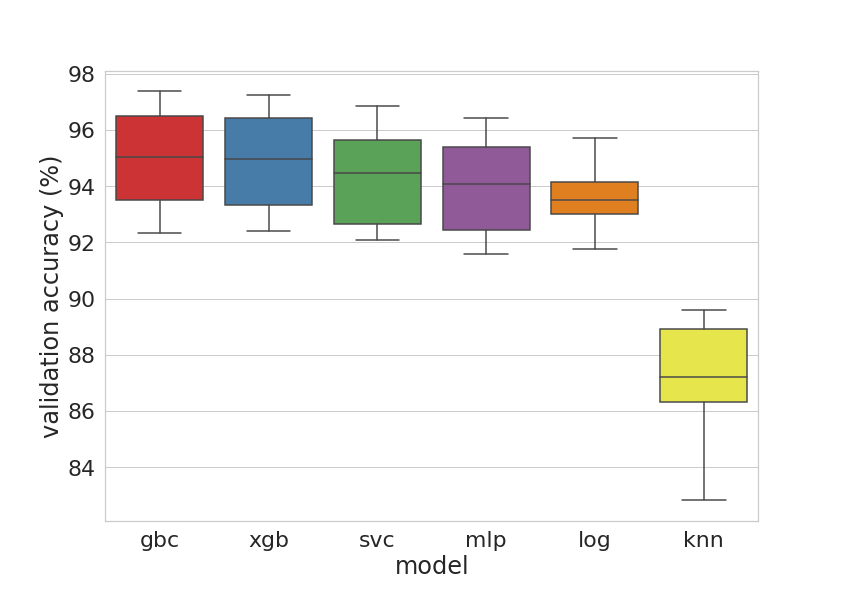
\includegraphics[width=8cm]{output/model_performance.png} & 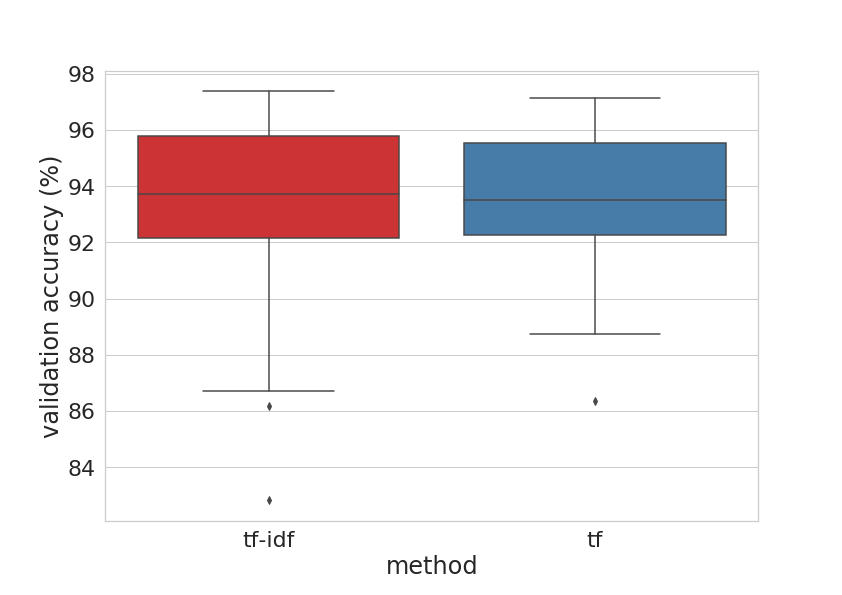
\includegraphics[width=8cm]{output/method_performance.png} \\
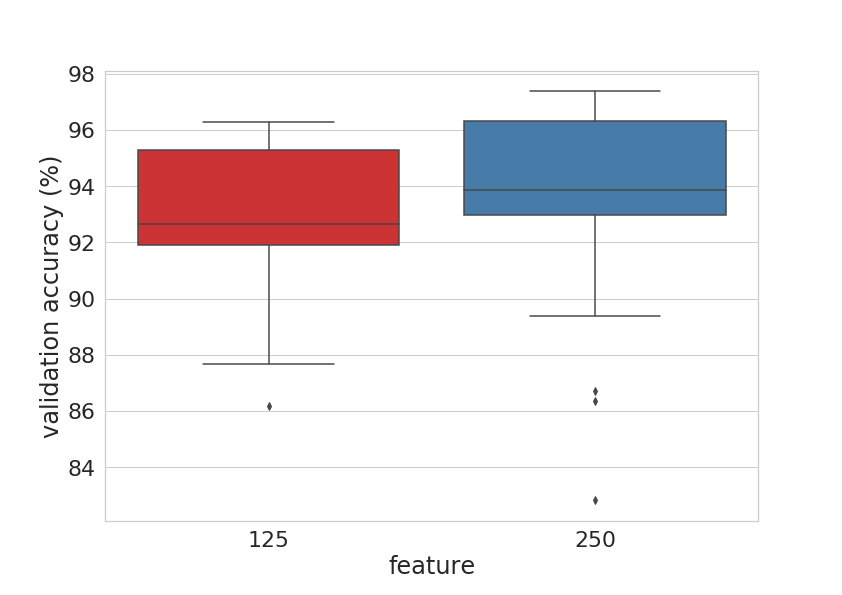
\includegraphics[width=8cm]{output/feature_performance.png} & 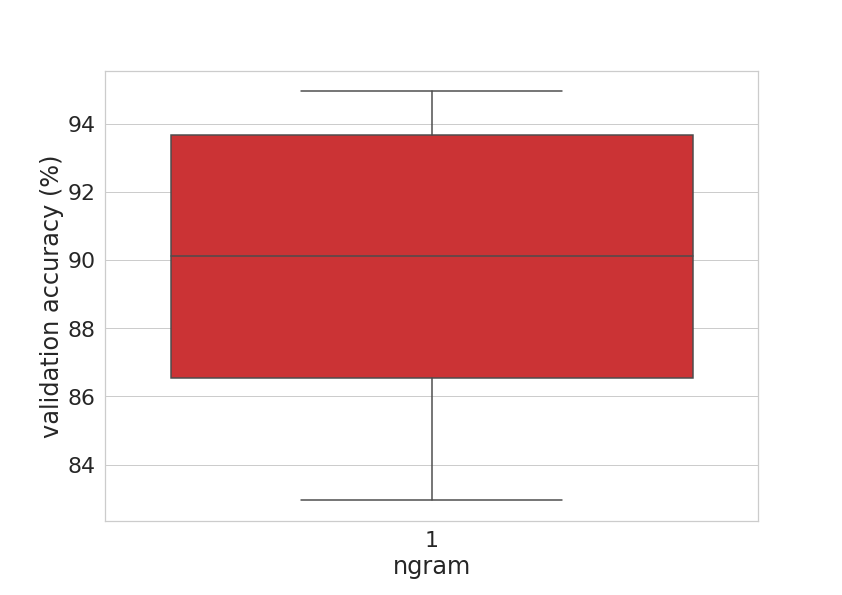
\includegraphics[width=8cm]{output/ngram_performance.png} \\
\end{tabular}
\end{center}
\caption{The influence on the accuracy of varied models, feature extraction methods, feature sizes and $n$-grams is demonstrated.}\label{fig:influenceparams}
\end{figure}

\subsubsection{Accuracy Performances}

The parameter combinations leading in the best five accuracy performances are shown in the table \ref{tab:accperf} below.

\begin{table}[h]
\begin{center}
\begin{tabular}{| l | l | c | c | c | c |}
\hline
Model & Method & Feature & $n$-gram & \thead{Accuracy on \\ test set (\%)} & \thead{Accuracy on \\ validation set (\%)} \\
\hline
knn & TF & 5,000 & 1 & 94.83 & 94.94 \\
knn & TF-IDF & 1,000 & 1 & 93.96 & 94.20 \\
knn & TF-IDF & 5,000 & 1 & 91.27 & 92.07	 \\
\hline 
\end{tabular}
\end{center}
\caption{Parameter combinations leading in the best three accuracies.}\label{tab:accperf}
\end{table}

\clearpage
\subsubsection{Detailed Results}

Detailed results on achieved accuracies, model hyper parameters and other varied parameters can be found on the \href{https://github.com/benjaminperucco/udacity-nano-mle/blob/master/5%20Capstone/2%20Project/3_postprocessing.ipynb}{Github repository}. 

\subsection{Justification}

Except for the knn model, we see very good performances leading to accuracies well above 90\%. This is in line with the finding of Ahmed et al. \cite{bib:ahmed-2017}. Even tough a much smaller feature size is used in this study, accuracies are similar or even better (250 vs. $\geq$ 1,000). The tree based models (gradient boosting \cite{bib:gbc} and XGBoost \cite{bib:xgb}) work best and lead to the best three accuracies (see table \ref{tab:accperf}). Ahmed et al. \cite{bib:ahmed-2017} found that a LSVM method is optimal.\\

\noindent It can be observed that both feature extraction methods TF and TF-IDF lead to almost equivalent results with a slight advantage for the TF-IDF method. Also, there seems to be almost a tie between the tested feature sizes (125 vs. 250). To save computational ressources, one should choose a feature size as low as practical. Furthermore, a unigram model leads to better results than a bigram model. The difference is quite significant as seen in figure \ref{fig:influenceparams}. 

\clearpage
\section{Conclusion} 

\subsection{Reflection}\label{chap:reflection}

Machine learning models are able to classify articles into two class labels of truthful and fake articles really well. It can be shown that an accuracy of 96\% can be achieved. But one has to ask the question what the methodology has been to decide which article is fake and which article is truthful. For example all truthful articles are from Reuters and fake articles were classified by Politifact. Even though this methodology is consistent for the set of articles analyzed in this work, it does not necessarily mean that new and unseen articles from other sources (others than Reuters for example) can be classified equally well by a machine learning model. This is one of the fundamental remaining question to be answered in a further study.

\subsection{Improvement}

Further investigations can be done in order to achieve an even better classification and increase training and prediction computation speed:

\begin{itemize}
\item{With such a large corpus of 44,898 documents, it can be difficult to achieve a text processing that is clean from text not related to the article (for example hyperlinks, references to twitter accounts, etc.). A second thorough investigation must dive deeper into the news articles to remove any unwanted stuff that remained from the present text processing implemented.}
\item{The methodology of article classification has to be reviewed and one has to clarify how well the classification performs on completely different sources of news articles (as mentioned in chapter \ref{chap:reflection}).}
\item{Calculating the correlation between features and focusing on features with low correlation could help to reduce the number of features and thus save compuation cost. The same could be achieved by applying principal component analysis (PCA).}
\end{itemize}

\clearpage
\begin{thebibliography}{9}
\bibitem{bib:fakenews} Fake news, December 30, 2020, wikipedia.org, \\\href{https://en.wikipedia.org/wiki/Fake_news}{\texttt{https://en.wikipedia.org/wiki/Fake\_news}}
\bibitem{bib:ahmed-2017} Ahmed H., Traore I., Saad S. (2017) Detection of Online Fake News Using N-Gram Analysis and Machine Learning Techniques. In: Traore I., Woungang I., Awad A. (eds) Intelligent, Secure, and Dependable Systems in Distributed and Cloud Environments. ISDDC 2017. Lecture Notes in Computer Science, vol 10618. Springer, Cham. \\\href{https://doi.org/10.1007/978-3-319-69155-8_9}{\texttt{https://doi.org/10.1007/978-3-319-69155-8\_9}}
\bibitem{bib:ahmed-2018} Ahmed, H, Traore, I, Saad, S. Detecting opinion spams and fake news using text classification, Security and Privacy, 2018, \\\href{https://doi.org/10.1001/spy2.9}{\texttt{https://doi.org/10.1001/spy2.9}}
\bibitem{bib:kaggle} Fake and real news dataset, December 30, 2020, kaggle.com, \\\href{https://www.kaggle.com/clmentbisaillon/fake-and-real-news-dataset}{\texttt{https://www.kaggle.com/clmentbisaillon/fake-and-real-news-dataset}}
\bibitem{bib:stemming} Stemming, December 30, 2020, wikipedia.org, \\\href{https://en.wikipedia.org/wiki/Stemming}{\texttt{https://en.wikipedia.org/wiki/Stemming}}
\bibitem{bib:sagemaker} Amazon SageMaker, December 30, 2020, amazon.com, \\\href{https://aws.amazon.com/sagemaker}{\texttt{https://aws.amazon.com/sagemaker}}
\bibitem{bib:scikit-learn} scikit-learn - machine learning in Python, December 30, 2020, scikit-learn.org, \\\href{https://scikit-learn.org/stable}{\texttt{https://scikit-learn.org/stable}}
\bibitem{bib:xgb} Amazon SageMaker - XGBoost Algorithm, December 30, 2020, amazon.com, \\\href{https://docs.aws.amazon.com/sagemaker/latest/dg/xgboost.html}{\texttt{https://docs.aws.amazon.com/sagemaker/latest/dg/xgboost.html}}
\bibitem{bib:knn} scikit-learn - k-nearest neighbors vote classifier, December 30, 2020, scikit-learn.org, \\\href{https://scikit-learn.org/stable/modules/generated/sklearn.neighbors.KNeighborsClassifier.html}{\texttt{https://scikit-learn.org/stable/modules/generated/\\sklearn.neighbors.KNeighborsClassifier.html}}
\bibitem{bib:svm} scikit-learn - c-support vector classification, December 30, 2020, scikit-learn.org, \\\href{https://scikit-learn.org/stable/modules/generated/sklearn.svm.SVC.html}{\texttt{https://scikit-learn.org/stable/modules/generated/\\sklearn.svm.SVC.html}}
\bibitem{bib:log} scikit-learn - logistic regression classifier, December 30, 2020, scikit-learn.org, \\\href{https://scikit-learn.org/stable/modules/generated/sklearn.linear_model.LogisticRegression.html}{\texttt{https://scikit-learn.org/stable/modules/generated/\\sklearn.linear\_model.LogisticRegression.html}}
\bibitem{bib:gbc} scikit-learn - gradient boosting for classification, December 30, 2020, scikit-learn.org, \\\href{https://scikit-learn.org/stable/modules/generated/sklearn.ensemble.GradientBoostingClassifier.html}{\texttt{https://scikit-learn.org/stable/modules/generated/\\sklearn.ensemble.GradientBoostingClassifier.html}}
\bibitem{bib:mlp} scikit-learn - multilayer perceptron classifier, December 30, 2020, scikit-learn.org, \\\href{https://scikit-learn.org/stable/modules/generated/sklearn.neural_network.MLPClassifier.html}{\texttt{https://scikit-learn.org/stable/modules/generated/\\sklearn.neural\_network.MLPClassifier.html}}
\end{thebibliography}

\end{document}